%%%%%%%%%%%%%%%%%%%%%%%%%%%%%%%%%%%%%%%%%%%%%%%%%%%%%%%%%%%%%%%%%%%%
%% I, the copyright holder of this work, release this work into the
%% public domain. This applies worldwide. In some countries this may
%% not be legally possible; if so: I grant anyone the right to use
%% this work for any purpose, without any conditions, unless such
%% conditions are required by law.
%%%%%%%%%%%%%%%%%%%%%%%%%%%%%%%%%%%%%%%%%%%%%%%%%%%%%%%%%%%%%%%%%%%%

\documentclass{beamer}
\usetheme[faculty=law,logoPath=./,logo=fudan_logo_vector.eps]{fibeamer}
\usepackage[utf8]{inputenc}
\usepackage{fontspec}
\setsansfont[Scale=MatchLowercase,Mapping=tex-text]{Calibri}
\setmonofont[Scale=MatchLowercase]{Courier New}  
\usepackage[
  % main=english, %% By using `czech` or `slovak` as the main locale
                %% instead of `english`, you can typeset the
                %% presentation in either Czech or Slovak,
                %% respectively.
    czech, 
    slovak,english, %% The additional keys allow foreign texts to be
]{babel}        %% typeset as follows:
%%
%%   \begin{otherlanguage}{czech}   ... \end{otherlanguage}
%%   \begin{otherlanguage}{slovak}  ... \end{otherlanguage}
%%
%% These macros specify information about the presentation
\title{Anisotropic in-plane thermal conductivity observed in multilayer silicene} %% that will be typeset on the
%% \subtitle{} %% title page.
\author{Yang Zhou}
%% These additional packages are used within the document:
\usepackage{ragged2e}  % `\justifying` text
\usepackage{booktabs}  % Tables
\usepackage{tabularx}
\usepackage{tikz}      % Diagrams
\usetikzlibrary{calc, shapes, backgrounds}
\usepackage{amsmath, amssymb}
\usepackage{url}       % `\url`s
\usepackage{listings}  % Code listings
\usepackage{color}

\frenchspacing
\begin{document}
\uselanguage{english}
\frame{
\maketitle \\
{\color{white} \today}
}


\begin{frame}<beamer>
  \frametitle{Outline} %%\thesection
  \tableofcontents
\end{frame}

\section{Introduction}
\begin{frame}[label=lists]{Introduction}

  \begin{enumerate}
    \item Silicene multilayer structure  has potential  in  thermalelectric field of quantum confinement and surface effects
          \begin{itemize}
            \item reduce thermal conductivity remarkably
          \end{itemize}
          \begin{itemize}
            \item remain the electric conductivity remain at a relatively high level
          \end{itemize}
          \begin{itemize}
            \item  thermalelectric figure of merit $ZT=\frac{S^2 \sigma T}{\kappa}$ could be optimized
          \end{itemize}

    \item Lack of study of thermaleletric properties of low-dimensional materials with interaction of covalent type
          \begin{itemize}
            \item they has large surface reconstruction while Van der Waals(vdW) type has not.
          \end{itemize}

  \end{enumerate}
  \bigskip
  \justifying

\end{frame}


\section{Structures}
\begin{frame}{Structures}
  \framesubtitle{Multilayer Silicenes}%
  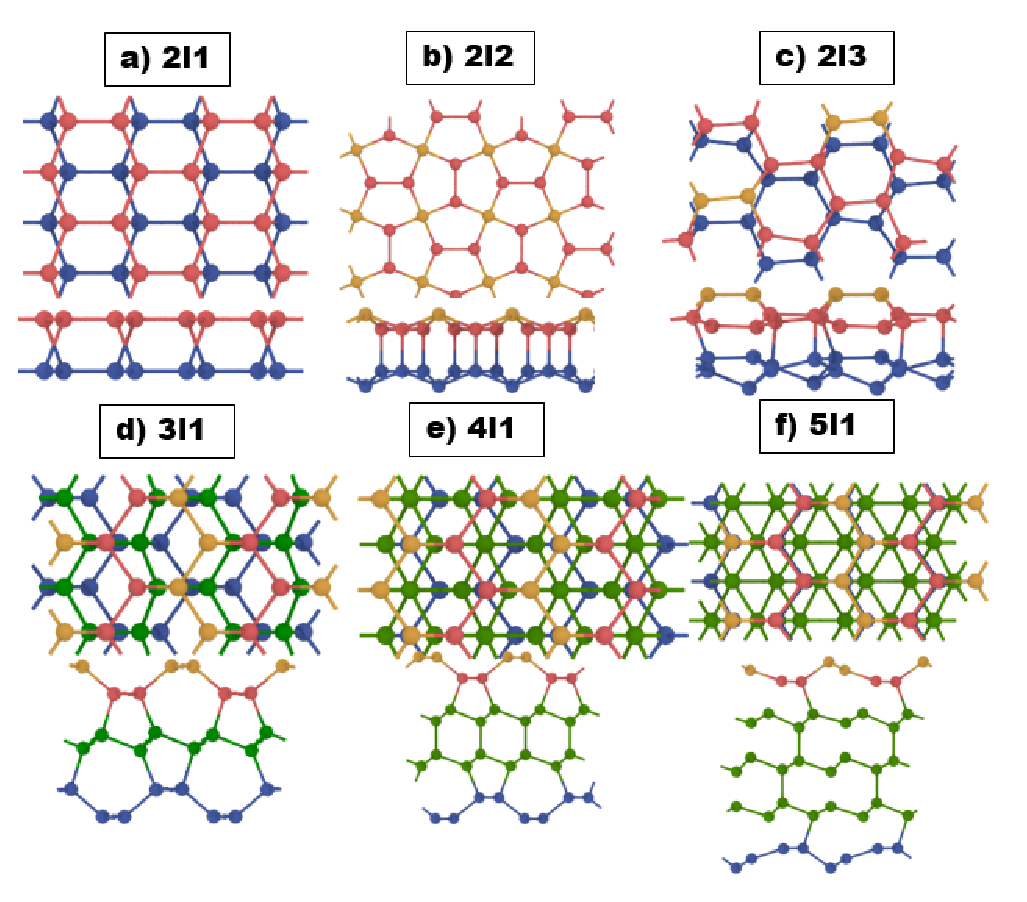
\includegraphics[width=\textwidth]{images/structures}
\end{frame}

\section{Thermal Conductivity Result}

\begin{frame}{TC Calculation}
  \framesubtitle{Boltzmann Transportation Theory}%

  \begin{columns}[onlytextwidth]
    \column{1\textwidth}
    The thermal conductivity tensor could be calculated with

    \begin{equation}
      \kappa^{\alpha\beta} = \sum_{k \sigma}{c_{k \sigma}v^{\alpha}_{k \sigma}v^{\beta}_{k \sigma}\tau_{k \sigma}} \label{eq:kappasum}
    \end{equation}

    Where $c_{k \sigma}$ means heat capacity of phonon mode $k \sigma$, $v^{\alpha}$ present for mode group velocity and $\tau_{k \sigma}$ is phonon lifetime. The heat capacity  could be computed with Eq.(\ref{eq:cv}) .

    \begin{equation}
      c_{k \sigma}=\frac{\hbar \omega_{k \sigma} }{V} \frac{\partial f(\omega_{k \sigma},T)}{\partial T} \label{eq:cv}
    \end{equation}

    Where $ f(\omega,T)=1/(exp(\frac{\hbar \omega}{k_b T})-1)$ is Bose-Einstein distribution function.


  \end{columns}

\end{frame}


\begin{frame}{Length dependence of TC}
  \begin{columns}[onlytextwidth]
    \column{.4\textwidth}
    The fitting line is obtained with $\kappa = \kappa_\infty (1-e^{-\frac{L}{L_c}})$. \\
    The letter z/a in the legend mean the transport direction is zigzag/armchair.
    \column{.6\textwidth}
    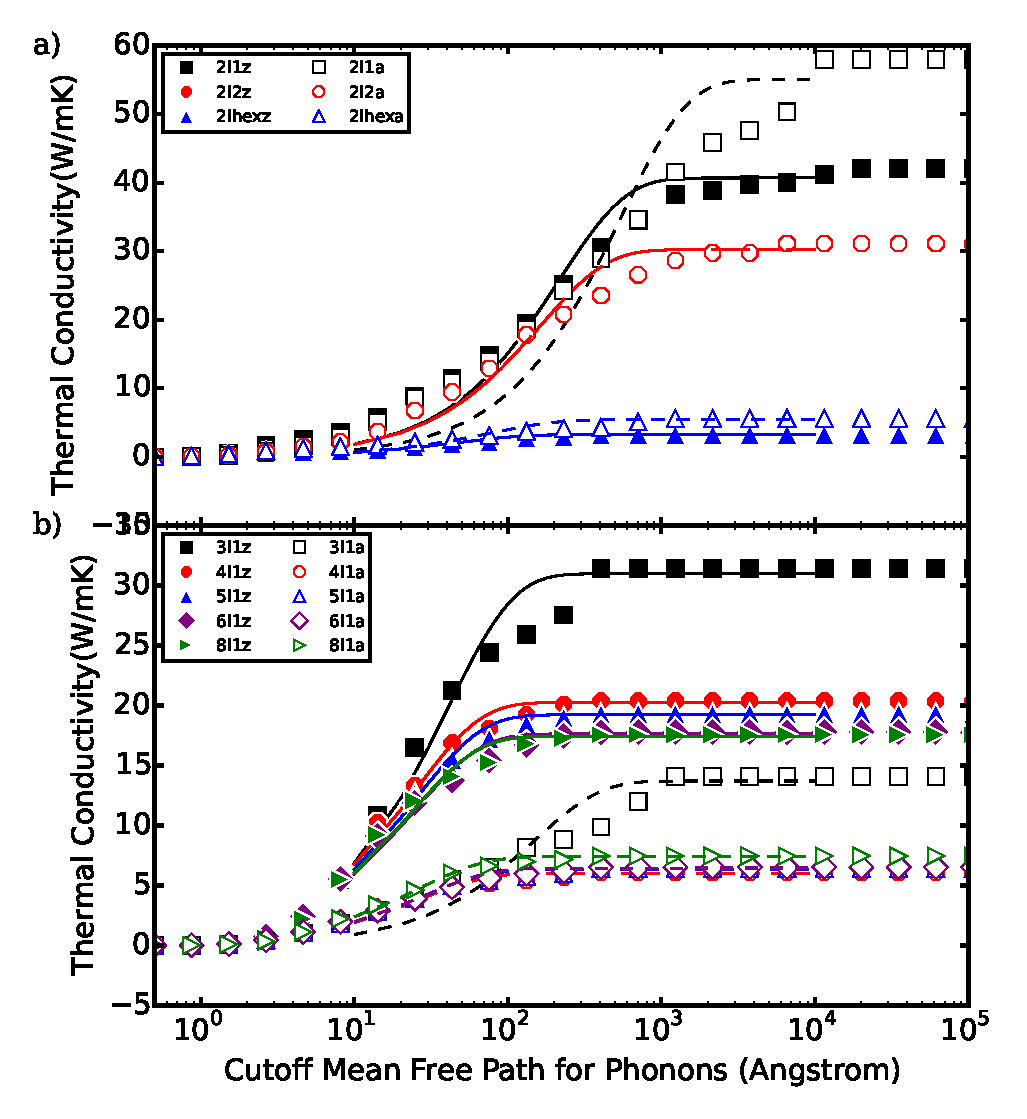
\includegraphics[width=\textwidth]{images/tc_length_sheng}


  \end{columns}

\end{frame}


\section{Anisotropy of Thermal Conductivity}
\begin{frame}{Anisotropy of Thermal Conductivity}
  \framesubtitle{Converged TC of varible structures}%
  $ \chi=|\kappa_{z,\infty}-\kappa_{a,\infty} |/max⁡(\kappa_{z,\infty}-\kappa_{a,\infty} ) \times 100 \%$
  \begin{table}[!b]
    {\carlitoTLF % Use monospaced lining figures
      \begin{tabular}{ccccccc}
            & Minimal period
            & $\kappa_{z,\infty}$
            & $\kappa_{a,\infty}$
            & $\chi$
            & $Cv_{z}$
            & $Cv_{a}$                                                           \\
        \toprule
        2l1 & $1 \times 1$             & 42.10 & 57.92 & 27.31\% & 165.8 & 166.7 \\
        2l2 & $\sqrt{2}\times\sqrt{2}$ & 31.11 & 31.11 & 0    \% & 38.44 & 38.44 \\
        2l3 & $2 \times 2$             & 3.311 & 5.624 & 41.13\% & 22.42 & 22.42 \\
        3l1 & $2 \times 1$             & 31.44 & 14.05 & 55.29\% & 52.22 & 52.46 \\
        4l1 & $2 \times 1$             & 20.37 & 6.114 & 69.98\% & 37.71 & 37.89 \\
        5l1 & $2 \times 1$             & 19.33 & 6.419 & 66.78\% & 29.17 & 29.32 \\
        6l1 & $2 \times 1$             & 17.78 & 6.527 & 63.29\% & 23.73 & 23.86 \\
        8l1 & $2 \times 1$             & 17.56 & 7.461 & 57.51\% & 17.26 & 17.36 \\
        \bottomrule
      \end{tabular}
    }

    \caption{
      Minimal period of the structures,thermal conductivity, anisotropy and heat capacity}
  \end{table}

\end{frame}


\begin{frame}{Length dependence of Anisotropy}
  \small
  \begin{columns}[onlytextwidth]
    \column{\textwidth}
    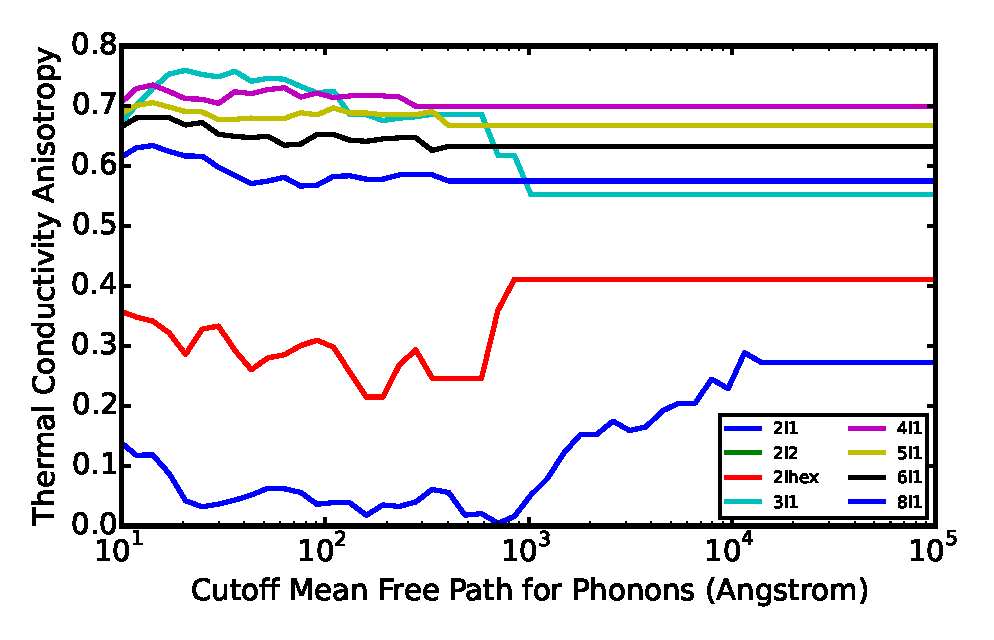
\includegraphics[width=\textwidth]{images/chi}


  \end{columns}

\end{frame}

\begin{frame}{Frenquency dependence of TC}
  \begin{figure}[b]
    \begin{columns}
      \small
      \column{\textwidth}
      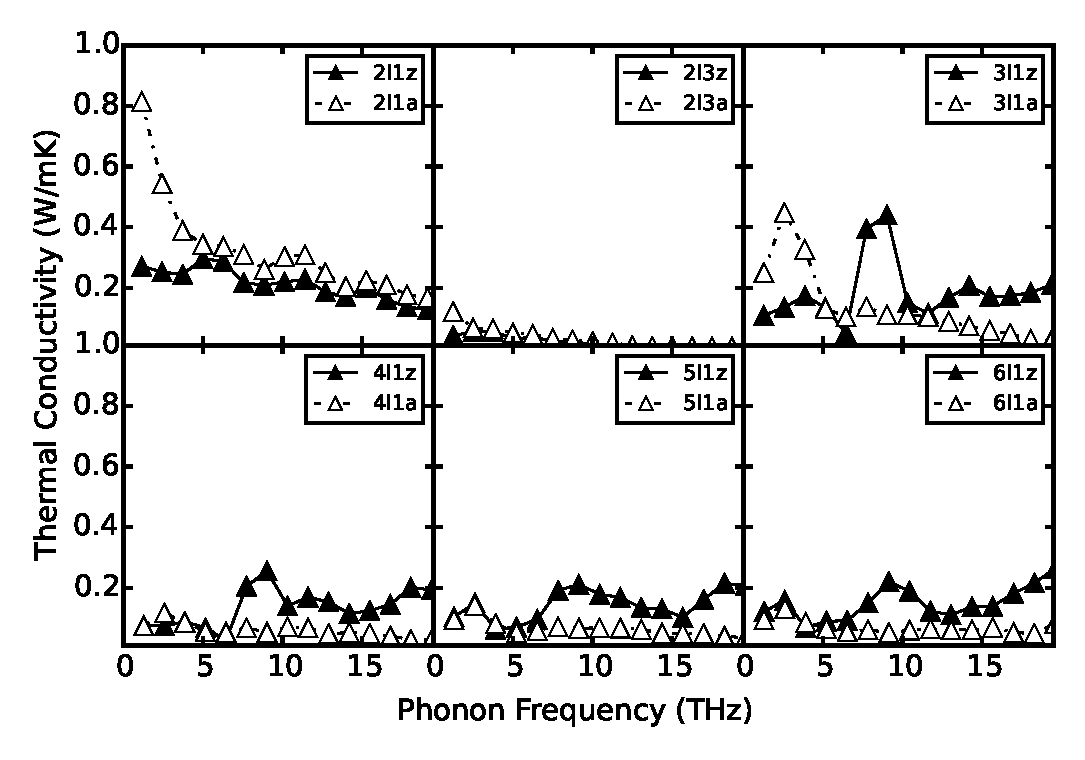
\includegraphics[width=\textwidth]{images/tc_freq}
      \caption{\label{fig:freq} The contribution of thermal conductivity from different frequency }
    \end{columns}
  \end{figure}
\end{frame}


\section{Scattering Contribution of Anisotropy}
\begin{frame}{Scattering Contribution of Anisotropy}
  \framesubtitle{Phonon Lifetime}%
  \begin{columns}[onlytextwidth]
    \column{1\textwidth}
    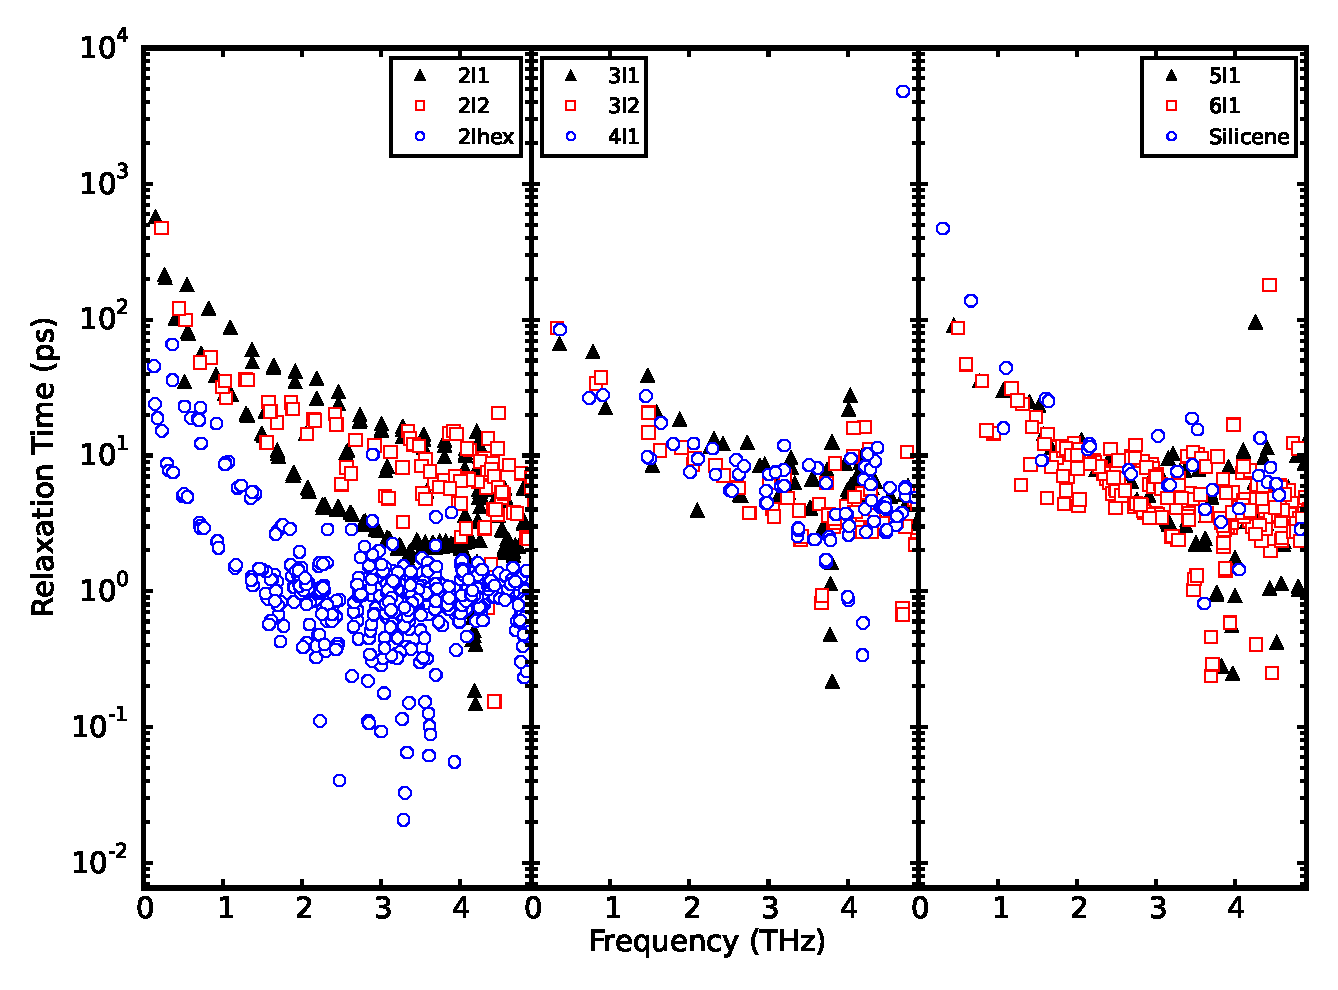
\includegraphics[width=\textwidth]{images/tau}

  \end{columns}
\end{frame}


\section{Localization Contribution of Anisotropy}
\begin{frame}{Localization Contribution of Anisotropy}
  \framesubtitle{ Group Velocity}%

  \begin{figure}[h]
    \centering

    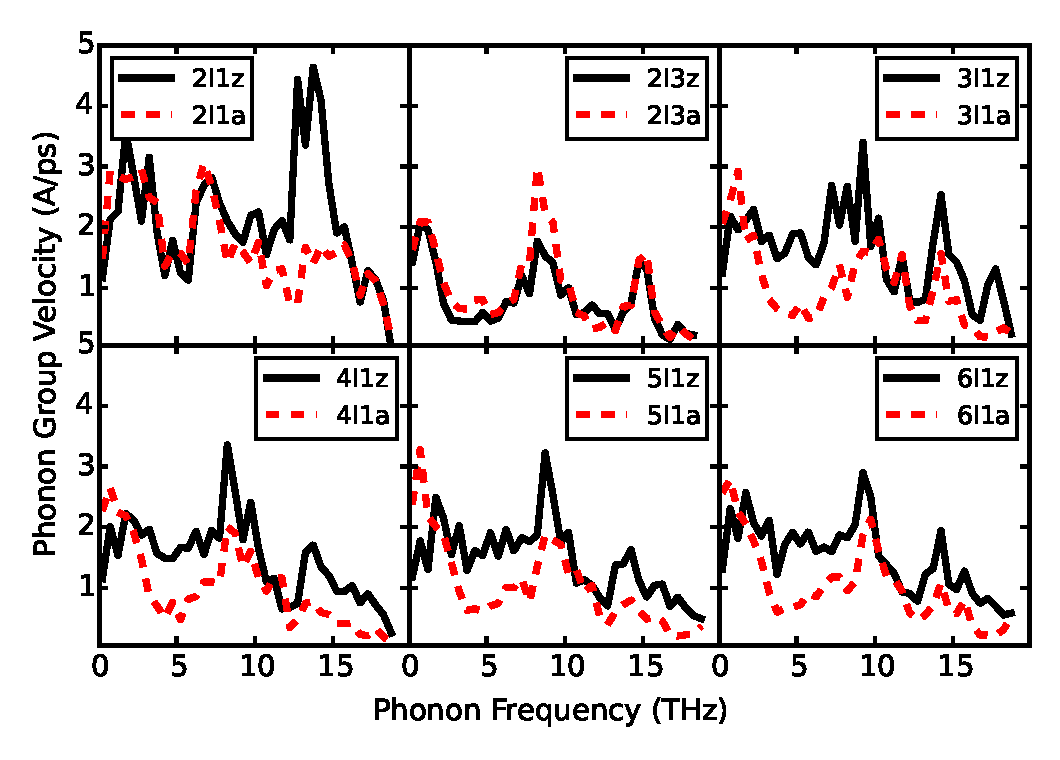
\includegraphics[width=.8\textwidth]{images/gv}
  \end{figure}
\end{frame}

\begin{frame}{Localization Contribution of Anisotropy}
  \framesubtitle{ Phonon Transmission}%
  \small
  $\Theta(\omega)= Tr(\mathbf{\widetilde{k}}_{a\alpha} Im(\mathbf{g}_{\alpha\alpha}) \mathbf{\widetilde{k}}_{\alpha a}\mathbf{G}_{a b}^*\mathbf{\widetilde{k}}_{b\beta}Im(\mathbf{g}_{\beta\beta})\mathbf{\widetilde{k}}_{\beta b}\mathbf{G}_{b a} )$
  \begin{figure}[h]
    \centering
    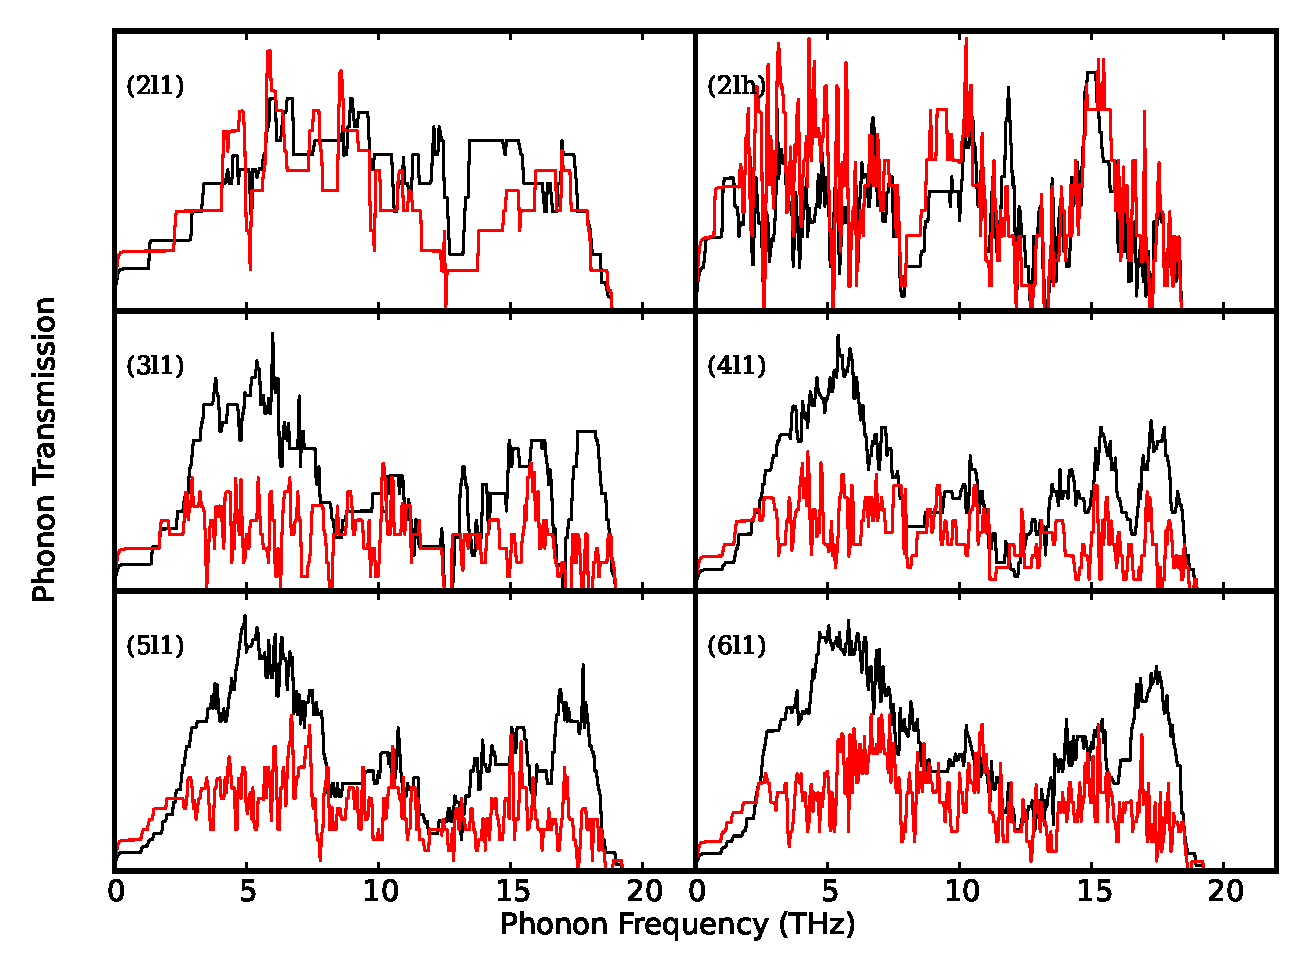
\includegraphics[width=.8\textwidth]{images/transmission}
  \end{figure}
\end{frame}





\section{Conclusion}
\begin{frame}[label=lists]{Conclusion}

  \begin{enumerate}
    \item layer = 2L
          \begin{itemize}
            \item The anisotropy mainly comes from scattering
          \end{itemize}
          \begin{itemize}
            \item Surface reconstruction affects the magnitude and anisotropy a lot.
          \end{itemize}
    \item layer >= 3L
          \begin{itemize}
            \item The anisotropy mainly comes from localization
          \end{itemize}
          \begin{itemize}
            \item Group velocity and Dispertion
          \end{itemize}
          \begin{itemize}
            \item Transmission
          \end{itemize}
  \end{enumerate}
  \bigskip
  \justifying

\end{frame}


\frame{
\title{Thanks for your attention !}
\maketitle \\
{\color{white} \today
}
}
\end{document}
